\documentclass{article}
\usepackage{arxiv}

\usepackage[utf8]{inputenc}
\usepackage[english, russian]{babel}
\usepackage[T1]{fontenc}
\usepackage{url}
\usepackage{booktabs}
\usepackage{amsfonts}
\usepackage{nicefrac}
\usepackage{microtype}
\usepackage{lipsum}
\usepackage{lmodern}
\usepackage{graphicx}
\usepackage{natbib}
\usepackage{doi}



\title{Итеративное улучшение тематической модели с обратной связью от пользователя}

\author{ Горбулев Алексей Ильич \\
	\texttt{gorbulev.ai@phystech.edu} \\
	\And
	Алексеев Василий Антонович \\
	\texttt{vasiliy.alekseyev@phystech.edu} \\
	\And
    Воронцов Константин Вячеславович \\
    \texttt{vokov@forecsys.ru} \\
}
\date{}

\renewcommand{\undertitle}{}
\renewcommand{\shorttitle}{Итеративное улучшение тематической модели с обратной связью от пользователя}

%%% Add PDF metadata to help others organize their library
%%% Once the PDF is generated, you can check the metadata with
%%% $ pdfinfo template.pdf
%%% \hypersetup{
%%% pdftitle={A template for the arxiv style},
%%% pdfsubject={q-bio.NC, q-bio.QM},
%%% pdfauthor={David S.~Hippocampus, Elias D.~Striatum},
%%% pdfkeywords={First keyword, Second keyword, More},
%%% }

\begin{document}
\maketitle

%%% термин «мусорная» взята из изначального задания, возможно, стоит изменить на стилистический нейтральный термин, но пока этого делать не стал, чтобы не нарушать изначальное задание

%%% some issues will be fixed later

\begin{abstract}
	В работе представлен метод тематического моделирования с использованием обратной связи от пользователя. Обратная связь заключается в определении принадлежности темы, полученной при тематическом моделировании, к одной из трёх категорий: релевантная, нерелевантная, <<мусорная>>. Основная задача состоит в улучшении базовой модели, которое заключается в выделении новых релевантных тем при сохранении выделенных тем и уменьшении числа <<мусорных>> тем. В работе предлагается решение с использованием библиотек тематического моделирования и регуляризаторов сглаживания и декоррелирования. Вычислительный эксперимент проводится на текстовой коллекции, основанной на новостях сайта Lenta.ru.
\end{abstract}

\keywords{Тематическое моделирование \and ARTM \and Обработка естественного языка}

\section{Введение}
Одним из методов анализа текстов, который применяется в том числе в социологических исследованиях \citep{DIMAGGIO2013570} и активно развивается в последнее время \citep{10031921}, является тематическое моделирование.
Тематическая модель помогает оценить вероятность принадлежности текста к каждой из полученных тем.
Именно вероятностное тематическое моделирование использовалось при исследовании распространения информации о пандемии COVID-19 в Хорватии \citep{pandemic2021}, освещения в средствах массовых информации Литвы климатических изменений \citep{climate2021}.

Однако задача построения вероятностной тематической модели имеет бесконечно много решений \citep{bigartm} вследствие некорректной постановки.
С целью ограничения количества решений вводятся регуляризаторы. 
Например, декорреляция способствует улучшению когерентности тем \citep{artm2}, разреживание способствует обнулению части элементов матриц.

В то же время, не все темы могут оказаться \textit{релевантными} в контексте проводимого исследования.
Часть документов, которая по содержанию релевантны, могут быть отнесены как к \textit{нерелевантной} теме, которая дублирует по содержанию релевантную, так и к \textit{<<мусорной>>} теме, которая не имеет отношения к исследованию, что негативно влияет на качество исследования.

Целью данного исследования является построение обновляемой тематической модели с использованием обратной связи от пользователя, найденные релевантные темы которой охватывают в совокупности большую часть коллекции документов.
Пользователь относит каждую из тем к одной из трёх категорий: релевантные, нерелевантные и <<мусорные>> темы. Улучшение модели, которое основывается на пользовательской разметке, способствует сохранению ранее найденных релевантных тем и выделению пользователем новых релевантных тем, а также уменьшению числа <<мусорных тем>>.

%%% Объектом данного исследования являются методы тематического моделирования, алгоритмы пользовательской разметки тем и итеративного обновления моделей.

Для решения задачи используются в том числе и методы аддитивной регуляризации тематических моделей (ARTM), реализованные в библиотеках с открытым кодом \texttt{BigARTM} и \texttt{TopicNet}, которые включают в себя регуляризаторы декоррелирования и сглаживания. Именно подход ARTM способствует оптимизации моделей по сумме нескольких критериев \citep{artm}, что помогает учитывать особенности коллекции текстов и ограничить количество решений задачи тематического моделлирования. В качестве набора текстовых данных используется коллекция, основанная на новостях, опубликованных на сайте Lenta.ru в период с $1999$ по $2019$ годы.

\section{Постановка задачи}

%%% возможно, постановка не совсем корректна и не совсем отображает глубину этой задачи

Пусть $D$ — коллекция текстов, $W$ — множество термов.
Среди термов могут быть как ключевые слова, так и словосочетания \citep{artm2}.
Каждый документ $d \in D$ представим в виде последовательности $n_d$ термов $\left( w_1, \dots, w_{n_d} \right)$ из множества $W$ \citep{artm}.
Предполагается конечное множество тем $T$.
Коллекция документов $D$ рассматривается выборка из дискретного распределения $p(w, d, t)$ на конечном множестве $W \times D \times T$ \citep{artm2}.
 Согласно формуле полной вероятности и гипотезе условной независимости, распределение термов в документе $p(w \mid d)$ описывается вероятностной смесью распределений термов в темах $\varphi_{wt} = p(w \mid t)$ с весами $\theta_{td} = p (t \mid d)$ следующим образом: \citep{bigartm}
 $$p(w \mid d) = \sum \limits_{t \in T} p(w \mid t, d) p(t \mid d) = \sum \limits_{t \in T} p (w \mid t) p (t \mid d) = \sum \limits_{t \in T} \varphi_{wt} \theta_{td}$$
 Задача тематического моделирования состоит в нахождении по коллекции документов $D$ параметров $\varphi_{wt}$ и $\theta_{td}$, приближающих частотные оценки условных вероятностей $\widehat{p} (w \mid d)$.
 Так как $|T|$ обычно намного меньше, чем $|W|$ и $|D|$, то находится низкоранговое стохастическое матричное разложение \citep{artm2}
 $$F \approx \Phi \Theta$$ 
 где $F = {(\widehat{p}_{wd})}_{|W| \times |D|}$ — матрица частот терм в документах, $\Phi = {(\varphi_{wt})}_{|W| \times |T|}$ — матрица термов тем, $\Theta = {(\theta_{td})}_{|T| \times |D|}$ — матрица тем документов.

Предполагается $T_i$ — множество тем на итерации $i \in \mathbb{N}$,  $T_i^1 \subset T_i$ — подмножество релевантных тем с точки зрения пользователя, $T_i^2 \subset T_i$ — подмножество нерелевантных тем с точки зрения пользователя, $T_i^3 \subset T_i$ — подмножество <<мусорных>> тем с точки зрения пользователя, при этом $T_i = \sqcup_{k = 1}^3 T_i^k$, $M_i$ — состояние модели на итерации $i$.
Тогда итеративное улучшение модели $M_i$ состоит в построении модели $M_{i + 1}$, такой, чтобы множество тем $T_{i + 1}$ удовлетворяло следующим требованиям:

$$T_i^1 \subset T_{i + 1}^1, \ \left| T_{i + 1}^3 \right| \leq \left| T_i^3 \right|$$

\section{Метод}

Предполагается при обучении новой модели $M_{i + 1}$ выполнить следующее:

\begin{enumerate}
    \item При инициализации матрицы $\Phi$ зафиксировать столбцы, соответствующие релевантным темам $T_i^1$;
    \item При обучении использовать аддитивную регуляризацию тематических моделей (ARTM):
    \begin{enumerate}
        \item Для уменьшения числа дублирующих друг друга тем использовать регуляризатор декоррелирования, действующий на незафиксированные столбцы матрицы $\Phi$, матрицу из которых обозначим через $\Phi_{new}$:
        $$R (\Phi_{new}) = -\frac{\tau}{2} \sum \limits_{t \in (T_i^2 \cup T_i^3)} \sum \limits_{s \in T_i^3 \setminus t} \sum \limits_{w \in W} \varphi_{wt} \varphi_{ws}$$
        \item Для улучшения интерпретируемости тем использовать регуляризаторы сглаживания и разреживания относительно $\Phi_{new}$.
    \end{enumerate}
\end{enumerate}

%%% TODO: Возможно, стоит подробнее рассказать о методе

\section{Вычислительный эксперимент}

%%% На данный момент есть только базовый вариант эксперимента
Целью данного вычислительного эксперимента является нахождение способа улучшения тематической модели.
После обучения базовой модели полученные темы распределяются пользователем на три категории: релевантные, нерелевантные, "мусорные".
Далее используется несколько метрик, в том числе разреженность.
%%% TODO: пока не упомняты когерентность, разреженность и другие важные метрики, но они будут важны для финального варианта.
Новая модель строится добавлением новых регуляризаторов и изменением параметров.
Сравнивается количество тем в каждой категории и новые значения метрик.

\subsection{Описание данных}

\texttt{Описан базовый вариант.}

Для обучения тематических моделей использовались новости, опубликованные на сайте Lenta.ru с $1$ января по $31$ марта $2002$ года.
Каждая из $5492$ новостей распределена по одной из $8$ макротем: <<Из жизни>>, <<Интернет и СМИ>>, <<Культура>>, <<Мир>>, <<Россия>>, <<Силовые структуры>>, <<Спорт>>, <<Экономика>>.
Далее происходит предобработка данных с помощью токенизации, лемматизации, выделения биграмм, приведения текста в формат, совместимым с библиотекой Vowpal Wabbit.
Каждая тема характеризуется пользователем по $5$ ключевым словам и $5$ ключевым биграммам.

%%% Подробнее будет со временем, кроме того, хотелось бы понять, достаточно ли приводить фрагменты текстов из макротем или же просто тем

\subsection{Базовая модель}

%%% К несчастью, с выделением коэффициентов регуляризаторов произошли проблемы, удивительно не обнаружить ничего, что было бы отличным от нуля, что на самом деле не так

В качестве базовой модели $M_0$ используется тематическая модель с регуляризатором декоррелирования, применяемым относительно слов, прошедших лемматизацию
Всего используется $50$ специальных тем и $1$ фоновая.
Далее используется тематическая модель $M_1$, использующая регуляризаторы декоррелирования и сглаживания как для лемматизированных слов, так и для биграмм.

\subsection{Предварительные результаты}

Среди тем, предложенных базовой моделью, были выделены $27$ релевантных, $11$ нерелевантных и $12$ <<мусорных>> тем.
Добавление новых регуляризаторов декоррелирования и сглаживания как для лемматизированных слов, так и для биграмм, позволило выделить $2$ новые релевантные темы среди <<мусорных>>, а также сохранить все ранее выделенные релевантные темы.

%%% Код придётся так или иначе переделывать под новый эксперимент с новыми регуляризаторами, поэтому приводятся данные для базового эксперимента

\begin{center}
    \begin{tabular}{c|c|c|c|}
        Модель & $|T_1|$ & $|T_2|$ & $|T_3|$ \\
        \hline
        $M_0$ & $27$ & $11$ & $12$ \\
        $M_1$ & $29$ & $11$ & $10$
    \end{tabular}
\end{center}

\begin{figure}[h]
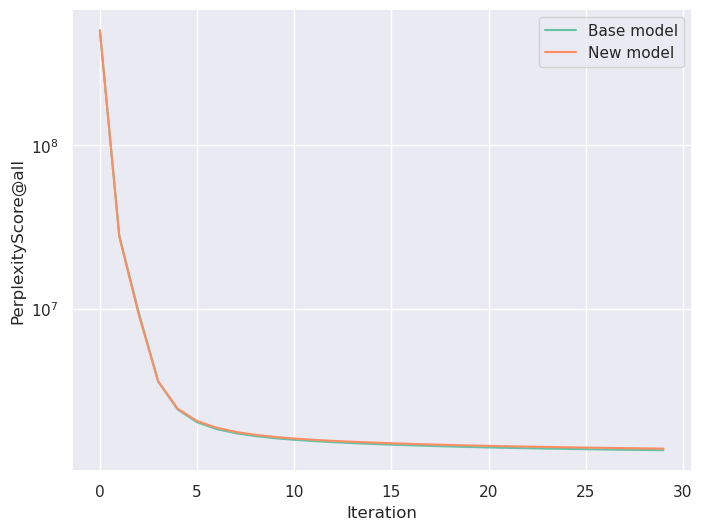
\includegraphics[width=9cm]{figures/perplexity_all.png}
\centering
\caption{Перплексия}
\end{figure}

\begin{figure}[h]
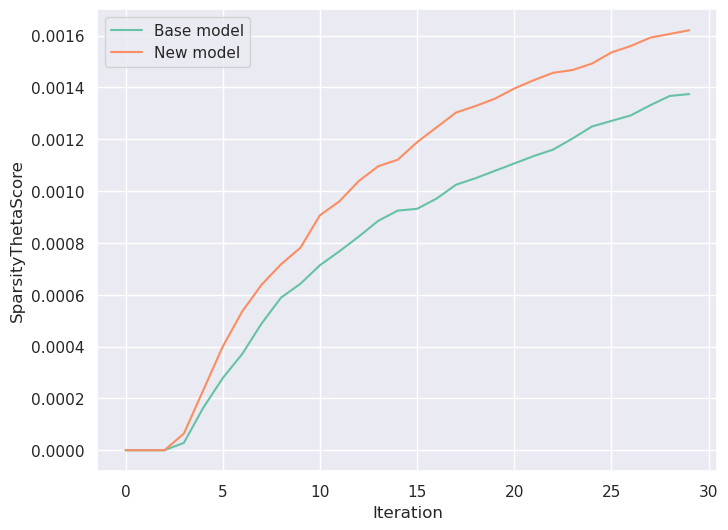
\includegraphics[width=9cm]{figures/sparsity_theta.png}
\centering
\caption{Разреженность матрицы $\Theta$}
\end{figure}

\begin{figure}[h]
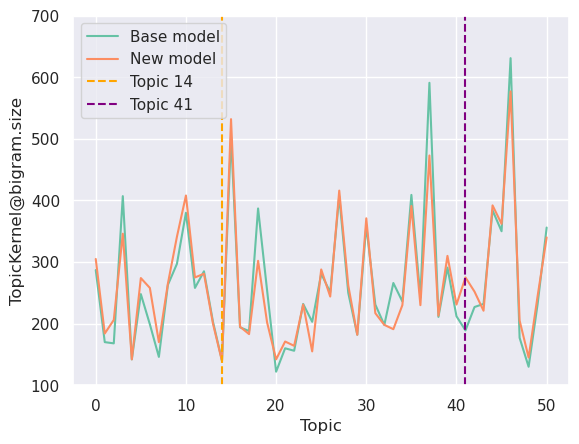
\includegraphics[width=9cm]
{figures/topickernel_bigram_size.png}
\centering
\caption{Итоговый размер ядер тем}
\end{figure}

Для новой модели разреженность выше, чем для базовой модели, что позволяет более точно определять темы с меньшим количеством возможных конфликтов. Изменились и размеры ядер тем, что отразилось и на теме $41$, признанной новой релевантной. При этом происходит крайне незначительная потеря перплексии, что является обычной ситуацией \citep{artm2}.

\bibliographystyle{plain}
\bibliography{Gorbulev2023TopicModels}

\end{document}